\chapter{Exercises}\label{ch:exercises}

\section{Turing Machines}

\begin{ex}
	Define an efficient 1-tape Turing Machine computing the function $\text{inverse}: \{0,1\}^* \to \{0,1\}^*$ such that $\text{inverse}(x)$ is the binary string obtained by flipping all bits in $x$, e.g. $\text{inverse}(01011)$ is 10100. Give the Turing Machine explicitly as a triple in the form $(\Gamma,Q,\delta)$.
\end{ex}

\begin{solution}
	The alphabet $\Gamma$ can be defined as $\{\start,\blank,0,1\}$, while the set of states $Q$ is $\{q_{\text{init}}, q_s, q_r\}$. The transition function is specified as follows:
	\begin{align*}
		(q_{\text{init}},\start) & \longmapsto (q_s,\start,S)             \\
		(q_s,\start)             & \longmapsto (q_2,\start,R)             \\
		(q_s,0)                  & \longmapsto (q_s,1,R)                  \\
		(q_s,1)                  & \longmapsto (q_s,0,R)                  \\
		(q_s,\blank)             & \longmapsto (q_r,\blank,S)             \\
		(q_r,\blank)             & \longmapsto (q_r,\blank,L)             \\
		(q_r,0)                  & \longmapsto (q_r,0,L)                  \\
		(q_r,1)                  & \longmapsto (q_r,1,L)                  \\
		(q_r,\start)             & \longmapsto (q_{\text{halt}},\start,S)
	\end{align*}
	In all the other cases (e.g. when the state is $q_{\text{init}}$ and the symbol is not $\start$, the behavior of the machine is not relevant, i.e., $\delta$ can be defined arbitrarily defined.
\end{solution}

\begin{ex}
	Define an efficient 2-tape Turing Machine accepting only words $w \in \{0,1\}^*$ having the same number of 0's and 1's. For example, 011100 is accepted and 101 is rejected. Give the Turing Machine explicitly as a triple in the form $(\Gamma,Q,\delta)$.
\end{ex}


\begin{solution}
	The general idea is that we write every 1 we encounter in the input tape into the working tape until we reach the end of the word. We then go back and move left on the working tape only when there is a matching 0 in the input tape.

	We take $\Gamma = \{\start,\blank,0,1\}$ for the alphabet, $Q = \{q_{\text{init}},q_{\text{halt}},q_r,q_l\}$ for the set of states and the transition function $\delta: Q \times \Gamma^2 \to Q \times \Gamma \times \{L,S,R\}^2$ as follows:

	\begin{align*}
		(q_{\text{init}},(\start,\start)) & \overset{\delta}{\longmapsto} (q_r,\start,(R,R))                                              \\
		(q_r,(0,\blank))                  & \longmapsto (q_r,\blank,(R,S))                                                                \\
		(q_r,(1,\blank))                  & \longmapsto (q_r,1,(R,R))                                                                     \\
		(q_r,(\blank,\blank))             & \longmapsto (q_l,\blank,(L,L))                                                                \\
		(q_l,(0,1))                       & \longmapsto (q_l,\blank,(L,L))                                                                \\
		(q_l,(1,1))                       & \longmapsto (q_l,1,(L,S))                                                                     \\
		(q_l,(\start,\start))             & \longmapsto (q_{\text{halt}},\start,(S,S))       & \success \text{same number of 0's and 1's} \\
		(q_l,(0,\start))                  & \longmapsto (q_l,\start,(S,S))                   & \fail \text{more 0's, the TM is stuck}     \\
		(q_l,(\start,1))                  & \longmapsto (q_l,1,(S,S))                        & \fail \text{more 1's, the TM is stuck}
	\end{align*}
\end{solution}

\begin{ex}
	Construct a deterministic TM of the kind you prefer, which decides a language $\lang{L}$ containing all the $w \in \binstrings$ such that between any pair of occurrences of $0$ in $w$ there's  an odd number of $1$s.
	Study the complexity of TM you have defined.
\end{ex}
\begin{solution}
	We define a 1-tape Turing Machine with alphabet $\Gamma = \{\start,\blank,0,1\}$ and with a set of states $Q = \{q_{\text{init}}, q_1, q_2, q_3, q_4, q_{halt}\}$. The transition function $\delta : Q \times \Gamma \to Q \times \Gamma \times \{ S,L,R \}$ is specified as follows:
	\begin{align*}
		(q_{init}, \start) & \overset{\delta}{\longmapsto} (q_1,\start,R)                \\
		(q_1,1)            & \longmapsto (q_1,1,R)                                       \\
		(q_1,0)            & \longmapsto (q_2,0,R)                                       \\
		(q_1,\blank)       & \longmapsto (q_{halt}, \blank, S) \quad \success \ w = 1^n  \\
		(q_2, 1)           & \longmapsto(q_3,1,R)                                        \\
		(q_2,0)            & \longmapsto(q_3,0,S)                                        \\
		(q_2,\blank)       & \longmapsto(q_{halt}, \blank,S) \quad \success w = 1^k0     \\
		(q_3, 1)           & \longmapsto (q_4,1,S)                                       \\
		(q_3, \blank)      & \longmapsto(q_{halt}, \blank,S)                             \\
		(q_3,0)            & \longmapsto (q_2,0,R) \quad \text{back to 1st 0 occurrence} \\
		(q_4, 1)           & \longmapsto (q_3,1,S) \quad \text{even n of 1s}             \\
		(q_4,0)            & \longmapsto (q_{halt},0,S) \quad \fail                      \\
		(q_4,\blank)       & \longmapsto (q_{halt}, \blank, S) \quad \success
	\end{align*}


	The TM has to go through the tape only one time, so the complexity is linear $O(n)$.
\end{solution}


\section{Undecidability and Rice's theorem}

\begin{ex}
	Prove the undecidability of the language
	\[
		\lang{L}_E =
		\{ \enc{\mathcal{M}} | \mathcal{M} \text{ is a TM and } \epsilon \in \lang{L}(\mathcal{M})\}
	\]
	by showing that (a) $\lang{L}_E$ is reducible to $\lang{L}_{halt}$ and (b) via Rice's Theorem.
\end{ex}
\begin{solution}
	As discussed in Section~\ref{sec:semantic-languages}, we look for a computable mapping $\phi$, which we define here as the function $\phi : \binstrings \times \binstrings \to \binstrings$ such that
	\[
		\phi (\alpha, x) = \epsilon \iff \mathcal{M}_{\alpha} \text{ halts on input } x \, .
	\]
	The TM corresponding to $\phi$ can be defined as follows: run $\mathcal{M}_{\alpha}$ on input $x$ and erase the output tape so that $\epsilon$ is yielded.

	If we assume $\mathcal{L}_E$ to be decidable, then there exists a Turing machine $\mathcal{M}_E$ such that for an input $(\alpha, x)$, it returns 1 if $\mathcal{M}_\alpha$ outputs $\varepsilon$ on input $x$ and returns 0 otherwise. \\
	We now define a TM $\mathcal{M}_{halt}$ which for an input $(\alpha,x)$ returns 1 if $\mathcal{M}_E(\phi(\alpha),x)$ returns 1 and returns 0 otherwise. Therefore, $\mathcal{M}_{halt}(\alpha,x)$ returns 1 if and only if $\alpha$ halts on $x$.

	We now show that $\mathcal{L}_E$ is undecidable by using Rice's theorem:
	\begin{itemize}
		\item $\mathcal{L}_E$ is not trivial: the ``constant" Turing machine which always outputs 1 is not it $\mathcal{L}_E$ and the ``constant" Turing machine which always outputs $\varepsilon$ is in $\mathcal{L}_E$.

		\item $\mathcal{L}_E$ is semantic: for two Turing machines $\mathcal{M}$ and $\mathcal{N}$ with $\enc{\mathcal{M}}$ in $\mathcal{L}_E$ and for all input $x$, $M$ and $\mathcal{N}$ have the same output, we must have $[N]$ in $\mathcal{L}_E$. If $\enc{\mathcal{M}}$ in $\mathcal{L}_E$, then it ouputs $\varepsilon$ for some input $x$ so by hypothesis, $\mathcal{N}$ must also output $\varepsilon$ for $x$ and therefore $\enc{\mathcal{N}}$ is in $\mathcal{L}_E$.
	\end{itemize}

	Therefore, we can apply Rice's theorem~\ref{thm:rice-thm} and conclude that $\mathcal{L}_E$ is undecidable. \qed


\end{solution}

\section{Polynomial-time computable problems}

How can we prove that an algorithm works in polynomial time?
We do that in 4 steps:

\begin{enumerate}
	\item We \emph{encode} the input as a binary string. Our analysis of the complexity of the algorithm will be given with respect to the length (call it $\ell$) of such a string.

	\item We prove that the number of instructions of the algorithm is \emph{bounded by a polynomial} in $\ell$.

	\item We argue that each instruction can be simulated by a Turing machine in polynomial time.

	\item We show that all \emph{`intermediate' data and results} of the algorithm are bounded by a polynomial in $\ell$.
\end{enumerate}


\begin{ex}[Linear search]
	Given a list $A = [a_1,\ldots,a_n]$ such that $\forall i,\ a_i \in \mathbb{N}$ return an index $i \in \{1,\ldots,n\}$ such that $A[i] = v$, where $v \in \mathbb{N}$, if any, otherwise return $-1$.
	Input: list $A$ and natural number $v$
	Output: natural number
	\label{ex:linear-search}
\end{ex}

\begin{solution}

	One algorithm solving is Exercise~\ref{ex:linear-search} is Algorithm~\ref{alg:linear-search}:

	\begin{algorithm}
		\caption{Linear Search}\label{alg:linear-search}
		\KwData{$A = [a_1,\ldots,a_n], v$}
		\KwResult{An index $i \in \{1,\ldots,n\}$ s.t. $A[i] = v$, if any, $-1$ otherwise}
		$i \gets 1$\;
		\While{$i \leq n$}{
			\If{$A[i] = v$}{
				\Return{$i$}\;
			}
			\Else{
				$i \gets i + 1$\;
			}
		}
		\Return{$-1$}\;
	\end{algorithm}
\end{solution}
(\emph{Input encoding}). In order to encode $A = [a_1,\ldots,a_n]$ as a binary string, we first need to encode its components $a_i$. For that, we can choose one standard encoding of the natural numbers in $\binstrings$. Let us write $\enc{a_i}$ for the encoding of $a_i$ in binary. Since using $n$ bits we can encode $2^n - 1$ (natural) numbers, the encoding of a number $a \in \mathbb{N}$ requires $\log a + 1$ bits\sidenote{Actually, we should take the floor of $\log a, \floor{\log{a}}$.}. Therefore, we have $|\enc{a_i}| = \log a_i + 1$. The next step is to understand how to encode the whole $A$. For that, we regard a list of elements $[b_1,\ldots,b_n]$ as a `pair of pairs' of the form $(((b_1,b_2),b_3),\ldots b_n)$. Recall that given a pair $(b_1,b_2)$ of bitstrings, we can define the string $\enc{(b_1,b_2)} \in \binstrings$ by first translating $(b_1,b_2)$ as the string $b_1\#b_2 \in \{0,1,\#\}$ and then encoding $b_1\#b_2$ as a string $\enc{(b_1,b_2)} \in \binstrings$. For the latter point, we simply map 0 to 00, 1 to 11, and \# to 01. As a consequence, we see that $|\enc{(b_1,b_2)}| = 2|b_1| + 2|b_2| + 2$. Now, given a list $[b_1,\ldots,b_n]$ of bitstring by regarding it as a pair $(((b_1,b_2),b_3),\ldots b_n)$, we see that we obtain an encoding $\enc{[b_1,\ldots,b_n]}$ of length $\sum_{i=1}^n 2|b_i|+2(n-1)$. Applying these general considerations to $A$ (and recalling that $|\enc{a_i}| = \log a_i + 1$), we obtain:

\[
	\enc{A} = \enc{[\enc{a_1},\ldots,\enc{a_n}]} \qquad |\enc{A}| = \sum_{i=1}^n 2(\log a_i + 1) + 2(n-1)
\]

Finally, we pair $A$ with $v$ (recall that both $A$ and $v$ are input of our algorithm), so $\enc{(\enc{A},\enc{v})}$ gives an encoding of the input of our algorithm in binary notation. Notice that
\[
	\ell = |\enc{(\enc{A},\enc{v})}| = 2\left(\sum_{i=1}^n 2(\log a_i + 1) + 2(n-1)\right) + 2(\log v + 1) + 2.
\]

We now move to step 2. The latter is straightforward. Our algorithm consists of:
\begin{itemize}[noitemsep,topsep=0pt,parsep=0pt,partopsep=0pt]
	\item 1 assignment ($i \leftarrow 1$).
	\item $n$ iteration of:
	      \begin{itemize}[noitemsep,topsep=0pt,parsep=0pt,partopsep=0pt]
		      \item[-] An inequality check ($i \leq n$).
		      \item[-] A conditional branching performing:
		            \begin{itemize}[noitemsep,topsep=0pt,parsep=0pt,partopsep=0pt]
			            \item[*] An equality check ($A[i] = v$),
			            \item[*] Either a return instruction or an assignment ($i \leftarrow i + 1$).
		            \end{itemize}
	      \end{itemize}
	\item 1 return instruction
\end{itemize}
Therefore, the number of the instruction is of the form $b + c \cdot n$, for suitable constants $b,c$, and thus it is bounded by a polynomial in $\ell$.

(\emph{TM simulation}).
In order to prove step 3, we have to argue that all the aforementioned instructions can be simulated by a TM in polynomial time. For instance, an equality check can be simulated as follows. Say we have two values $a$ and $b$ stored in different portions of a tape of a TM. In order to check whether $a$ is equal to $b$, the machine simply moves back and forth between $a$ and $b$ checking whether they are bitwise equal. This can be done in polynomial time with respect to the length of $a$ and $b$, provided that the `distance' between $a$ and $b$ in the tape is itself bounded by a polynomial in the length of $a$ and $b$. This will be indeed ensured by step 4. Similar arguments can be used to show that all other instructions can be simulated efficiently by a TM.

(\emph{Intermediate data/results size}).
Finally, in order to prove step 4 we simply observe that the only intermediate value computed by our algorithm is $i$, which can be at most $n$ (and therefore it is bounded by a polynomial in $\ell$).

\begin{ex}[Universal sink]
	Recall that a \emph{directed} graph is a pair $G = (V,E)$ where $V$ is a set of vertices and $E \subseteq V \times V$ is the `edge' relation between vertices. Notice that we do not require $E$ to be symmetric. We represent graphs using the so-called adjacency matrices. Formally, we regard graphs as pairs $(V,A)$ where $V = \{v_1,\ldots,v_n\}$ is a set of vertices and $A$ is an $n \times n$-matrix over $\{0,1\}$. Intuitively, $A$ encodes the edge relation according to the convention that $A_{i,j} = 1$ if and only if there is an edge from $v_i$ to $v_j$. A \emph{universal sink} is a vertex $v_i$ such that for all $j,k \leq n$ with $j \neq i$ we have
	\[
		A_{i,k} = 0 \qquad A_{j,i} = 1
	\]
	Notice that if a graph has a universal sink, then the latter is unique.
	Show that determining whether a graph has a universal sink is computable in polynomial time.
	\label{ex:universal-sink}
\end{ex}
\begin{solution}
	Let $G = (V,A)$ be a graph with $V = \{v_1,\ldots,v_n\}$. We design Algorithm~\ref{alg:universal-sink} to solve Exercise~\ref{ex:universal-sink}.
	The key observation is noticing that if $v_i$ is a universal sink, then the $i$-th row in $A$ contains only 0s, whereas the $i$-th column contains all 1s (except in the entry $A_{i,i}$). Graphically:

	\[
		\begin{pmatrix}
			          & i &                           \\
			          & 1 &                           \\
			          & 1 &                           \\
			          & 1 &                           \\
			i \quad 0 & 0 & 0 \quad 0 \quad 0 \quad 0 \\
			          & 1 &                           \\
			          & 1 &
		\end{pmatrix}
	\]

	Let us write $US(v)$ for the property ``$v$ is a universal sink''. Then, we see that for all vertices $v_j,v_k \in V$ we have that
	\[
		\begin{aligned}
			A_{j,k} = 1 & \implies \neg US(v_j); \\
			A_{j,k} = 0 & \implies \neg US(v_k).
		\end{aligned}
	\]

	We can thus proceed as follows. Let $POS$ be a list of potential universal sinks. Obviously, we begin assuming $POS = V$. We sequentially pick pairs of vertices $(v_i,v_j)$ in $POS$ and look at $A_{j,k}$. If $A_{j,k} = 1$, then we know that $v_j$ cannot be universal sink, and thus we remove it from $POS$. Otherwise, $A_{j,k} = 0$ meaning that $v_k$ cannot be universal sink, and thus we remove it from $POS$. Proceeding this way, we will end up with $POS$ containing a single vertex $v_i$. We then check whether $v_i$ is universal sink by checking whether the $i$-th row of $A$ contains 0s only, and whether the $i$-th column of $A$ contains all 1s (except for $A_{i,i}$). If we succeed then $v_i$ is a universal sink. Otherwise, there is no universal sink.

	\begin{algorithm}
		\caption{Universal Sink Detection}\label{alg:universal-sink}
		\KwData{$V = [v_1,\ldots,v_n], A$}
		\KwResult{An index $i \in \{1,\ldots,n\}$ s.t. $US(v_i)$, if any, $-1$ otherwise}
		$POS \gets [1,\ldots,n]$\;
		// We use only labels of vertexes
		$i \gets 1$\;
		$j \gets 2$\;
		\While{$j \leq n$}{
			\If{$A_{i,j} = 1$}{
				$POS = POS.remove(i)$\;
				$i \gets j$\;
				$j \gets j + 1$\;
			}
			\Else{
				$POS = POS.remove(j)$\;
				$j \gets j + 1$\;
			}
		}
		$i = POS.fst$\;
		// We have $POS = [i]$ for some $i$
		// Check row
		$j \gets 1$\;
		\While{$j \leq n$}{
			\If{$A_{i,j} = 0$}{
				$j \gets j + 1$\;
			}
			\Else{
				\Return{$-1$}\;
			}
		}
		// Check column
		$j \gets 1$\;
		\While{$j \leq n$}{
			\If{$A_{j,i} = 1$ or $j = i$}{
				$j \gets j + 1$\;
			}
			\Else{
				\Return{$-1$}\;
			}
		}
		\Return{$i$}\;
	\end{algorithm}

	Notice that we might have been more efficient in checking columns and rows. However, our implementation is closer to what we would do when programming a TM and makes our analysis easier.

	We now show that the above algorithm works in polynomial time. First, the encoding of the input is standard. The input, in fact, consists of a natural number $n$ (the number of vertices\footnote{Recall that we actually work with labels $1,\ldots,n$ of vertices, rather than with vertices themselves.}) and of an $n \times n$-matrix of bits. We encode the latter as a list made of $n$ elements each of which consisting of $n$ bits. Therefore, such an encoding has length $2n^2 + n - 1$. Pairing the latter with the encoding of $n$ (which has length $\log n$), we obtain an input of length $2(2n^2 + n - 1) + 2\log n + 1$.

	How many instructions our algorithm has? The first loop consists of $n-1$ iterations, each of which essentially consists of assignments, checking values of the matrix, and removing elements from a list. After that, we have loops for checking row and columns, which consist of $n$ iteration each (and thus a total of $2n$ iterations). Summing up, we have $3n - 1$ iterations, plus a fixed number of equality checking, assignments (plus arithmetic operations), and basic operations on lists. The algorithm thus has running time $O(n)$, and thus it is polynomial in $2(2n^2 + n - 1) + 2\log n + 1$.
	The last two points to prove in order to conclude that our algorithm runs in polynomial time
	are showing that each instructions can be simulated by a TM in polynomial time, and that
	all intermediate values/results have length polynomially bounded by the length of the input.
	The latter point is straightforward, whereas for the former we essentially proceed as in the solution of Exercise~\ref{ex:linear-search}.
\end{solution}

\begin{ex}[FP function]
	Given two strings $v,w$, determine whether $v$ is a substring of $w$, i.e., whether $w$ contains an exact occurrence of $v$.
\end{ex}

\begin{solution}
	\begin{algorithm}
		\caption{Substring Check}\label{alg:substring}
		\KwData{Strings $v,w$}
		\KwResult{True if $v$ is substring of $w$, False otherwise}
		$n \gets \text{size}(w)$\;
		$m \gets \text{size}(v)$\;
		$k \gets 0$\;
		\For{$i \in 0..n-1$}{
			\If{$v[k] = w[i]$}{
				$k \gets k + 1$\;
			}
			\Else{
				$k \gets 0$\;
			}
		}
		\Return{$k = m$}\;
	\end{algorithm}

	\textbf{Input Encoding:}
	Let $n$ be the number of distinct symbols in strings $v,w$. Each symbol requires $\log n + 1$ bits. Using alphabet $\Sigma = \{0,1,\#,@\}$ encoded as $\{00,01,11,10\}$, where:
	\begin{itemize}
		\item $\#$ separates characters
		\item $@$ separates strings
	\end{itemize}
	For $k = |v| + |w|$, total input size is:
	\[l = 2k(\log n + 1) + 2k + 2\]
	which is polynomial.

	\textbf{Basic Instructions Count:}
	Algorithm contains:
	\begin{itemize}
		\item Three initial assignments
		\item Loop with $n$ iterations containing:
		      \begin{itemize}
			      \item Equality check
			      \item Assignment and increment or
			      \item Assignment to zero
		      \end{itemize}
		\item Final equality check
	\end{itemize}
	Total instructions: $a + bn = \mathcal{O}(n)$ where $n < l$, thus polynomial in input size.

	\textbf{Intermediate Results:}
	Counter variables are bounded:
	\begin{itemize}
		\item $k$ ranges from $0$ to $|v|$
		\item $i$ ranges from $0$ to $|w|$
	\end{itemize}

	\textbf{Basic Operations:}
	All operations are polynomial-time on a Turing Machine:
	\begin{itemize}
		\item Assignment
		\item Increment
		\item Equality check
	\end{itemize}
\end{solution}


\begin{ex}[FP function]
	Given a list $L = [L_1,\ldots,L_n]$, return its inverse $[L_n,L_{n-1},\ldots,L_1]$.
\end{ex}

\begin{solution}
	\begin{algorithm}
		\caption{List Inversion}\label{alg:inversion}
		\KwData{List $L$ of length $n$}
		\KwResult{Inverted list $\text{Inv\_L}$}
		$k \gets \text{size}(L)$\;
		$j \gets 0$\;
		\For{$i \gets k-1$ \KwTo $0$}{
			$\text{Inv\_L}[j] \gets L[i]$\;
			$j \gets j + 1$\;
		}
		\Return{$\text{Inv\_L}$}\;
	\end{algorithm}

	\textbf{Input Encoding:}
	For natural numbers $L_i$, using alphabet $\Sigma = \{0,1,\#\}$ encoded as $\{00,01,11\}$:
	\[\text{length} = 2n(\log L + 1) + 2n\]
	where $\#$ separates elements.

	\textbf{Basic Instructions Count:}
	Total instructions: $c + na = \mathcal{O}(n)$, where $n$ is input size.

	\textbf{Basic Operations:}
	All operations are polynomial-time on TM:
	\begin{itemize}
		\item Assignment
		\item Increment
		\item Equality check
	\end{itemize}

	\textbf{Intermediate Results:}
	All variables polynomially bounded:
	\begin{itemize}
		\item $k$: input size
		\item $j$: ranges from $0$ to $k$
		\item $\text{Inv\_L}$: same size as input
	\end{itemize}
\end{solution}

\begin{ex}[FP function]
	Given two lists $L = [L_1,\ldots,L_n]$ and $P = [P_1,\ldots,P_n]$ of rational numbers, return their scalar product.
\end{ex}

\begin{solution}
	\begin{algorithm}
		\caption{Scalar Product}\label{alg:scalar}
		\KwData{Lists $L,P$ of rational numbers, length $n$}
		\KwResult{Scalar product of $L$ and $P$}
		$n \gets \text{size}(P)$\;
		$\text{dot} \gets 0$\;
		\For{$i \gets 0$ \KwTo $n$}{
			$\text{dot} \gets \text{dot} + L[i] \cdot P[i]$\;
		}
		\Return{$\text{dot}$}\;
	\end{algorithm}

	\textbf{Input Encoding:}
	Using alphabet $\Sigma = \{+,-,0,1,\#,@,/\}$ requiring 3 bits, where:
	\begin{itemize}
		\item $@$ separates lists
		\item $\#$ separates numbers
		\item $/$ separates numerator/denominator
		\item $+,-$ for signs
	\end{itemize}
	Rational numbers encoded as $\text{Sign}\ \text{num}/\text{den}$. Total length:
	\[3 \cdot 2 \cdot 2n(\log n + 1) + 3 \cdot 2n + 3\]

	\textbf{Basic Instructions Count:}
	Total instructions: $c + n$, polynomial in input length.

	\textbf{Basic Operations:}
	All operations polynomial-time on TM:
	\begin{itemize}
		\item Assignment
		\item Addition
		\item Multiplication
	\end{itemize}

	\textbf{Intermediate Results:}
	$\text{dot}$ is polynomially bounded by input size.
\end{solution}



\section{\NP~complete problems}

% Suppose clique is the following set: \[\text{CLIQUE} = \{(\mathcal{G}, k) \ | \ \text{ is an undirected graph containing a glique of size at least k }\}\]\\
% \textbf{Prove that clique is NP-complete} by showing that \(\kSAT{3} \leq_p \text{CLIQUE}\)\\
% \textit{Hint: consider any 3CNF F as a graph whose vertices are the occurrences of literals in F}
% \\
% \textbf{Solution}
% A clique is a subset \(W \leq V\) of its vertices such that any pair \(v,w \in W\) of distinct vertices is such that \(\{v,w\} \in E\) . In other words given an undirected graph a clique is a subset of this graph where all the vertices are connected.
% \begin{figure}[H]
% 	\centerline{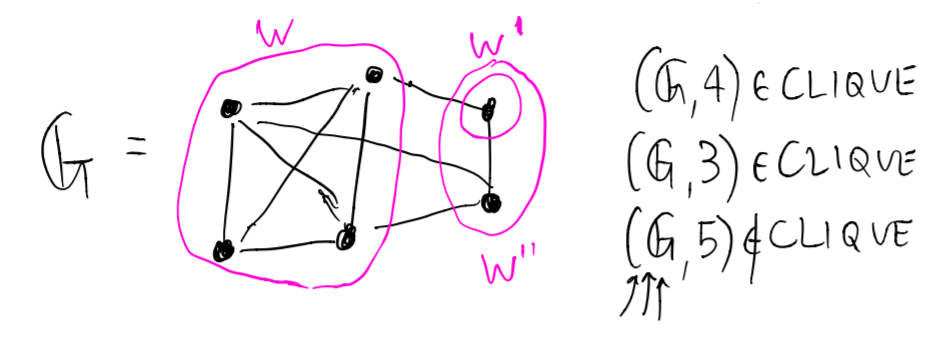
\includegraphics[scale=0.4]{figures/old/clique}}
% \end{figure}
% So \((\mathcal{G},4)\) belong to clique because in w (pink) I can see that I have at least 4 vertices which are all connected.  \((\mathcal{G},5)\) does not belong to clique because I can't find a subset of the graph where 5 vertices are all connected.\\
% The fact that clique in in NP is easy to prove: the certificate, as expected, is a subset \(W \subseteq V\) such that \(W\) has a k-CLIQUE. Indeed:
% \begin{itemize}
% 	\item Its size (which is its cardinality) is smaller than the one of \(\mathcal{G}\).
% 	\item checking that \(W\) is indeed a clique of size \(\geq\) to k can be done in quadratic time: it suffices to check that any pair of distinct vertices \(v,w \in W\) are connected by an edge.
% \end{itemize}
% About completeness, we want a reduction \(f\) such that for every 3CNF F, \(f(F)\) is a pair \((\mathcal{G}, k)\), and moreover \((\mathcal{G}, k) \in \text{CLIQUE}\) IFF F is satisfiable. So first of all we can observe that a natural way of turning CNFs into graphs consist in introducing a node for each literal in the CNF. So let's see what it means graphically
% \begin{figure}[H]
% 	\centerline{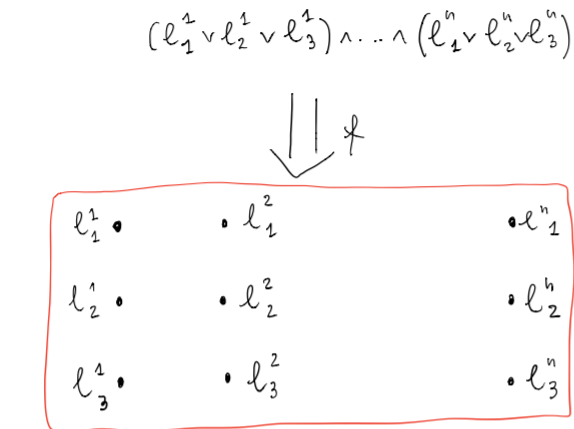
\includegraphics[scale=0.4]{figures/old/clique_1}}
% \end{figure}
% for every \(i \ne j\) and for every \(s,q \ in \{1,2,3\}\) we have an edge beween \(l_s^i\) and \(l_q^j\) iff the two literals are compatible from a logical point of view, namely iff they don't talk about the same variable in inconsistent ways (for example, we do not have an edge between \(x\) and \(\lnot x\) . \\
% The only missing ingredient in the proof is to prove that F is satisfiable IFF \(f(F)\) has a CLIQUE of size equal to the number of clauses in F:
% \begin{itemize}
% 	\item Suppose that F is satisfiable, then there is an assignment of truth value to the variables in F which makes the n clauses of F all \textbf{true}. This means that for every \(i \in \{1,...,n\}\) (the clause) there exists \(s \in \{1,2,3\}\) (the literals inside each clause) such that \(l_s^i\) is true in the assignment. All this literals then are pairwise consistent (i.e. it can't be that \(l_s^i=x \text{ and } l_q^j =\lnot x\) ), the nodes corresponding to these literals in \(f(F)\) are all linked by an edge. Hence \(f(F)\) is indeed a graph which has a clique of size n.
% 	\item Suppose that the graph \(f(F)\) has a clique of size n. It means that all columns of \(f(F)\) are "involved" in the clique (because there are no edges between nodes in the same column). There is thus a way of choosing for each clause in F one of its literals in such a way as to preserve logical consistency, and this, by definition of logical consistency, means that there is an assignment which makes all these literals true, since we have at least one literal for each clause. The formula F is satisfiable.
% \end{itemize}

\begin{theorem}
	The following set is NP-complete:
	\[\text{CLIQUE} = \{(\mathcal{G}, k) \mid \mathcal{G} \text{ is an undirected graph containing a clique of size at least } k \}\]
\end{theorem}

\begin{proof}
	First, we define a clique as a subset $W \subseteq V$ of vertices such that any pair $v,w \in W$ of distinct vertices satisfies $\{v,w\} \in E$. In other words, a clique is a subset where all vertices are pairwise connected.

	\textbf{CLIQUE} $\in$ \textbf{NP}:
	The certificate is a subset $W \subseteq V$ containing a $k$-clique because:
	\begin{itemize}
		\item $|W| \leq |\mathcal{G}|$
		\item Verifying $W$ is a clique of size $\geq k$ takes quadratic time: check each pair $v,w \in W$ for edge connectivity
	\end{itemize}

	\textbf{Reduction} $\kSAT{3} \leq_p \text{CLIQUE}$:
	We construct $f$ such that for every 3CNF formula $F$, $f(F) = (\mathcal{G}, k)$ where:
	\begin{itemize}
		\item Create a vertex for each literal occurrence in $F$
		\item For literals $l_s^i$ and $l_q^j$ where $i \neq j$ and $s,q \in \{1,2,3\}$:
		      Add edge $(l_s^i, l_q^j)$ iff literals are logically compatible
		      (e.g., no edge between $x$ and $\neg x$)
		\item Set $k$ equal to number of clauses in $F$
	\end{itemize}

	\textbf{Correctness}: $F$ is satisfiable iff $f(F)$ has a clique of size $k$ (number of clauses in $F$)

	($\Rightarrow$) If $F$ is satisfiable:
	\begin{itemize}
		\item Some truth assignment makes all $n$ clauses true
		\item For each clause $i \in \{1,\ldots,n\}$, $\exists s \in \{1,2,3\}$ where $l_s^i$ is true
		\item These literals are pairwise consistent (no $x$ and $\neg x$)
		\item Corresponding vertices form a clique of size $n$ in $f(F)$
	\end{itemize}

	($\Leftarrow$) If $f(F)$ has $n$-clique:
	\begin{itemize}
		\item Each column (clause) contributes one vertex (no edges within columns)
		\item Chosen literals preserve logical consistency
		\item This selection yields a satisfying assignment for $F$
		\item At least one true literal per clause implies $F$ is satisfiable
	\end{itemize}
\end{proof}

\begin{ex}
	Prove that the following language $L$ is in NP, where:
	\[L = \{(G,k) \mid G=(V,E) \text{ is a graph whose nodes can be partitioned into } \leq k \text{ independent sets}\}\]
	Equivalently:
	\[L = \{(G,k) \mid \exists N: V \to \{1,\ldots,k\} \text{ s.t. } \forall (u,v) \in E, N[u] \neq N[v]\}\]
	where $G = (V,E)$ is a graph and $k$ is a natural number.
\end{ex}

\begin{solution}
	\textbf{Certificate Structure:}
	Let $N: V \to \{1,\ldots,k\}$ be the certificate, where $N[v]$ represents the assigned number (color) for vertex $v$.

	\begin{algorithm}
		\caption{Graph Coloring Verifier}\label{alg:coloring}
		\KwData{Graph $G=(V,E)$, number $k$, assignment $N$}
		\KwResult{True if $N$ is valid $k$-coloring, False otherwise}
		\For{$(u,v) \in E$}{
			\If{$N[u] = N[v]$}{
				\Return{false}\;
			}
		}
		\Return{true}\;
	\end{algorithm}

	\textbf{Certificate Size:}
	\begin{itemize}
		\item $N$ contains $|V|$ numbers
		\item Each number is $\leq k$, requiring $\log k$ bits
		\item Total size: $\mathcal{O}(|V| \log k)$, polynomial in input size
	\end{itemize}

	\textbf{Verifier Complexity:}
	\begin{itemize}
		\item Checks each edge once
		\item Time complexity: $\mathcal{O}(|E|) = \mathcal{O}(|V|^2)$
		\item Polynomial in input size
	\end{itemize}

	Therefore, $L \in \textbf{NP}$.
\end{solution}

\begin{ex}[\kSAT{1}]
	Consider the following problem:
	\[
		\kSAT{1} = \{ \enc{A} | A \text{is a satisfiable 1CNF} \}
	\]
	To which complexity class does \kSAT{1} belong? Prove your claim.

	\begin{solution}
		\kSAT{1} belongs to the complexity class \P.

		\begin{algorithm}
			\caption{\kSAT{1}}\label{alg:onesat}
			\KwData{Matrix $A$ containing literals and their assignments}
			\KwResult{True if formula is satisfiable, False otherwise}
			$n \gets \text{size}(A)[0]$\;
			\For{$i \in 0..n$}{
				\For{$j \in 0..n$}{
					\If{$A[i][0] = A[j][0] \land A[i][1] \neq A[j][1]$}{
						\Return{false}\;
					}
				}
			}
			\Return{true}\;
		\end{algorithm}

		The input can be encoded as a list of literals, which may be negated. The encoding requires:
		\begin{itemize}
			\item Symbol to separate literals
			\item Symbol to denote negation
		\end{itemize}
		Using alphabet $\Sigma = \{0,1,\#,@\}$ encoded as $\{00,01,10,11\}$, where:
		\begin{itemize}
			\item $k$ is the number of different literals
			\item $n$ is the total number of literals
			\item $w < n$ is the number of negated literals
		\end{itemize}

		The total length of the input encoding is:
		\[l = 2(n(\log k + 1) + n + w)\]
		which is polynomial in the length of the input.

		The number of basic instructions is:
		\[c + b \cdot n^2\]
		which is polynomially bounded with respect to the length of the encoding of the input.

		Every basic instruction can be modeled by a Turing Machine that works in polynomial time. In particular, equality checking can be performed in polynomial time.

		The partial results (counter $i$) are natural numbers ranging from 0 to the input size, thus polynomially bounded by the length of the input encoding.

		Therefore, $\kSAT{1} \in \P$.
	\end{solution}
	%     1SAT belong to the complexity class P.
	% prove:
	% 1. Pseudocode:
	% n = size(A)[0]
	% for i in 0..n
	%  for j in 0..n
	%    if (A[i][0]==A[j][0] and A[i][1]!=A[j][1])
	%     return false
	% return true
	% 2. Encoding of the input:
	% the input can be encoded as a list of literals, that can be negated or not. We will need a symbol to separate the literals, one to negate a literal so in the end we will have the following alphabet {0,1,#,@} that encoded will be {00,01,10,11}. If k is the number of different literal and n the total number of literals and w is the total number of negated literal w<n, we will have that the total length of the input encoding will be l= 2 (n(log k +1)+ n+ w) that is polynomial in the length of the input.
	% 3. number of basic instruction:
	% The number of basic instruction is c+b*n^2 which is polynomially bounded with respect to the length of the encoding of the input.
	% 4. basic instruction polynomially bounded with respect to the length of the input encoding:
	% every instruction can be modeled by a TM that works in polynomial time, equality check, infact, can be done in polynomial time by a TM.
	% 5. Every partial result is polynomially bounded by the length of the input encoding:
	% i is a natural number that goes from 0 to the size of the input, so it is polynomially bounded.

	% Follow that 1SAT is in P.
	% \end{solution}

\end{ex}

\begin{ex}[\texttt{ONEINDSET}]
	Given \texttt{INDSET}, classify its subset \texttt{ONEINDSET} whose elements are pairs $(G,k)$ where:
	\begin{itemize}
		\item $G$ is an undirected graph where each node is in at most one edge
		\item $k$ is a natural number
	\end{itemize}
\end{ex}

\begin{solution}
	\textbf{Formal Definition:}
	\[\texttt{ONEINDSET} = \{(G,k) \mid \exists I \subseteq V: |I| \geq k \land \forall u,v \in I: (u,v) \notin E \]\[\land \forall u,v,w \in V: (u,v) \in E \implies (u,w) \notin E \text{ for } v \neq w\}\]

	\begin{theorem}
		Let $G=(V,E)$ be an undirected graph. If every $v \in V$ is contained in at most one edge, then $G$ has an independent set of size $|I| = |V|-|E|$.
	\end{theorem}

	\begin{proof}
		For each edge $(u,v) \in E$:
		\begin{itemize}
			\item Neither $u$ nor $v$ can be in any other edge by assumption
			\item Each edge eliminates exactly one vertex from potential independent set
			\item After excluding one vertex per edge, remaining vertices form independent set
			\item Size of independent set is $|V|-|E|$
		\end{itemize}
	\end{proof}

	\textbf{Complexity Classification:}
	\texttt{ONEINDSET} $\in$ P because:
	\begin{itemize}
		\item Can compute $|V|-|E|$ in polynomial time
		\item Compare with input $k$
		\item Return true iff $|V|-|E| \geq k$
	\end{itemize}
\end{solution}

\begin{ex}[\kCLIQUE{3}]
	We studied the problem \CLIQUE. You are required to classify the subset \kCLIQUE{3} of \CLIQUE consisting of all the pairs $(G,3)$. To which class does \kCLIQUE{3} belong?
\end{ex}

\begin{solution}
	THREECLIQUE belongs to the complexity class P.

	\begin{algorithm}
		\caption{\kCLIQUE{3}}\label{alg:3clique}
		\KwData{Graph $G = (V,E)$}
		\KwResult{True if graph contains a 3-clique, False otherwise}
		\For{$i \in V$}{
			\For{$j \in V$}{
				\For{$k \in V$}{
					\If{$(i,j) \in E \land (i,k) \in E \land (j,k) \in E$}{
						\Return{true}\;
					}
				}
			}
		}
		\Return{false}\;
	\end{algorithm}

	The input graph $G=(V,E)$ has $V$ encoded as a natural number and $E$ as pairs of natural numbers, with separator symbol $\#$ between natural numbers. Using alphabet $\Sigma = \{0,1,\#\}$ encoded as $\{00,01,11\}$, the total bits required are:
	\[l = 2(2\cdot|E|(\log n + 1) + 2|E| + (\log|V| + 1) + 1) = \mathcal{O}(|E|) = \mathcal{O}(|V|^2)\]

	With three nested loops iterating over $V$, the number of basic instructions is:
	\[c + b|V|^3 = \mathcal{O}(|V|^3)\]
	which is polynomial in the length of the input encoding.

	The most complex basic operation (checking if a pair is connected by an arc) runs in:
	\[\mathcal{O}(|E|) = \mathcal{O}(|V|^2) = \mathcal{O}(l)\]
	which is polynomial with respect to the input encoding size.

	Variables $i$, $j$, $k$ are natural numbers with maximum size $\log|V| + 1$ bits, which is polynomially bounded with respect to the input encoding size.

	Therefore, THREECLIQUE $\in$ P.


	% THREECLIQUE belong to the class P.
	% 1. Pseudocode
	% for i in V
	%  for j in V
	%   for k in V
	%    if (i,j) in E and (i,k) in E and (j,k) in E
	%     return true
	%   return false
	% 2. encoding the input
	% The input is G=(V,E). V can be encoded as a natural number, while E as pairs of natural numbers. We need a symbol # to separate the different natural numbers so our alphabet will be {0,1,#} that encoded will be {00,01,11}. The total bits that we need will be:
	% l= 2(2*|E|(log(n)+1) + 2|E| + (log V +1) +1)= O(|E|)= O(|V|^2)
	% 3. number of basic instruction:
	% we have three innested loop from 1 to V, so the total number of instruction is c+b|V|^3= O(|V|^3) which is polynomial in the length of the encoding of the input.
	% 4. basic instruction TM polynomially bounded
	% The only non-trivial instruction is checking if a pair is connected by an arc, which can be done in O(|E|)=O(|V|^2) = O(l) which is polynomial with respect to the size of the encoding of the input.
	% 5. partial data polynomially bounded 
	% i,j,k are natural number, their maximum size will be (log |V| +1) bit which is polynomially bounded with respect to the size of the encoding of the input.
\end{solution}

\begin{ex}[kSAT{4}]
	Consider the following problem:
	\[
		\kSAT{4} = \{ \enc{A} | A \text{is a satisfiable 4CNF} \}
	\]
	To which complexity class does \kSAT{1} belong? Prove your claim.

	to which complexity class does \kSAT{4} belong? Prove your claim.
\end{ex}
\begin{solution}
	\kSAT{4} is \NP-complete. We prove this in two steps:

	\textbf{1. \kSAT{4} $\in$ NP}

	We have \kSAT{4} = $\{A \mid \exists P \text{ such that } A(P)=\text{true}\}$, where $P$ is the certificate consisting of a truth assignment for each variable. The length of $P$ is polynomial with respect to the length of $A$. The verifying Turing Machine needs only to substitute the truth values in $A$, which can be done in polynomial time. Therefore, \kSAT{4} $\in$ NP.

	\textbf{2. \kSAT{3} $\leq_p$ \kSAT{4}}

	Problem definitions:

	\kSAT{3}:
	\begin{itemize}
		\item Input: Formula $A$
		\item Output: 1 iff $A$ is satisfiable and in 3CNF
	\end{itemize}

	\kSAT{4}:
	\begin{itemize}
		\item Input: Formula $A$
		\item Output: 1 iff $A$ is satisfiable and in 4CNF
	\end{itemize}

	The reduction \kSAT{3} $\leq_p$ \kSAT{4} means that $A \in$ \kSAT{3} iff $M(A) \in$ \kSAT{4}.

	\textbf{Reduction:} For each clause of the form $(A \lor B \lor C)$, create two clauses:
	\[(A \lor B \lor C \lor D) \land (A \lor B \lor C \lor \neg D)\]
	where $D$ is a new variable. This makes $D$'s truth value irrelevant to the satisfiability of the 4CNF formula. The reduction runs in polynomial time as we only add one new variable per clause.

	\textbf{Correctness:}

	($\Rightarrow$) If $A \in$ \kSAT{3}: Let $(A \lor B \lor C)$ be satisfiable. Then both $(A \lor B \lor C \lor D)$ and $(A \lor B \lor C \lor \neg D)$ are satisfiable by construction, as $D$'s value is irrelevant.

	($\Leftarrow$) If $M(A) \in$ \kSAT{4}: If $(A \lor B \lor C \lor D) \land (A \lor B \lor C \lor \neg D)$ is satisfiable, since we have both $D$ and $\neg D$ in different clauses, their values are irrelevant. Therefore, $(A \lor B \lor C)$ must be satisfiable in \kSAT{3}.

	Since \kSAT{3} is NP-complete and we have shown both \kSAT{4} $\in$ NP and \kSAT{3} $\leq_p$ \kSAT{4}, we conclude that \kSAT{4} is NP-complete.
\end{solution}


\begin{ex}[\kSAT{2}]
	Consider the following problem:
	2SAT = {A|A is a satisfiable 2CNF}
	To which complexity class does 2SAT belong? Prove your claim.
\end{ex}
\begin{solution}
	This is a quite complex problem to solve, but it has been solve and 2SAT belong to P. The dimonstration is based on the fact that I can rewrite (A or B) as ((notA => B) and (notB => A))
\end{solution}

\begin{ex}[\NODECOVER]
	see exercise sheet \#TODO place it here
	%     \begin{figure}[H]
	% 	\centerline{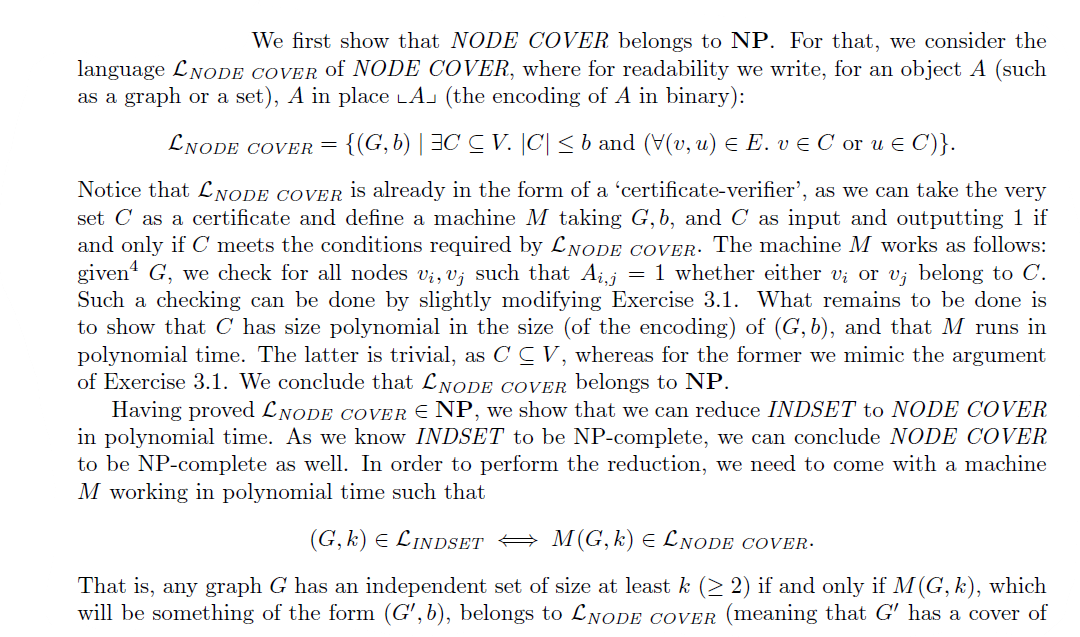
\includegraphics[scale=0.6]{figures/old/Nodecover1}}
	% \end{figure}
	% \begin{figure}[H]
	% 	\centerline{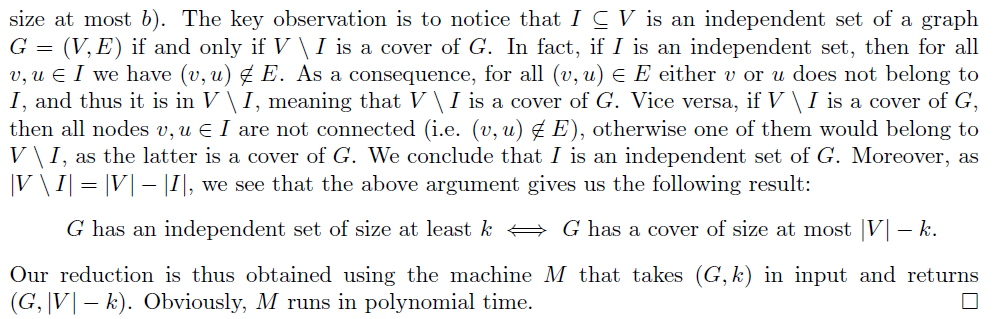
\includegraphics[scale=0.8]{figures/old/Nodecover2}}
	% \end{figure}
\end{ex}
\begin{ex}[\texttt{SET PACKING}]
	see exercise sheet \#TODO place it here
	%     \begin{figure}[H]
	% 	\centerline{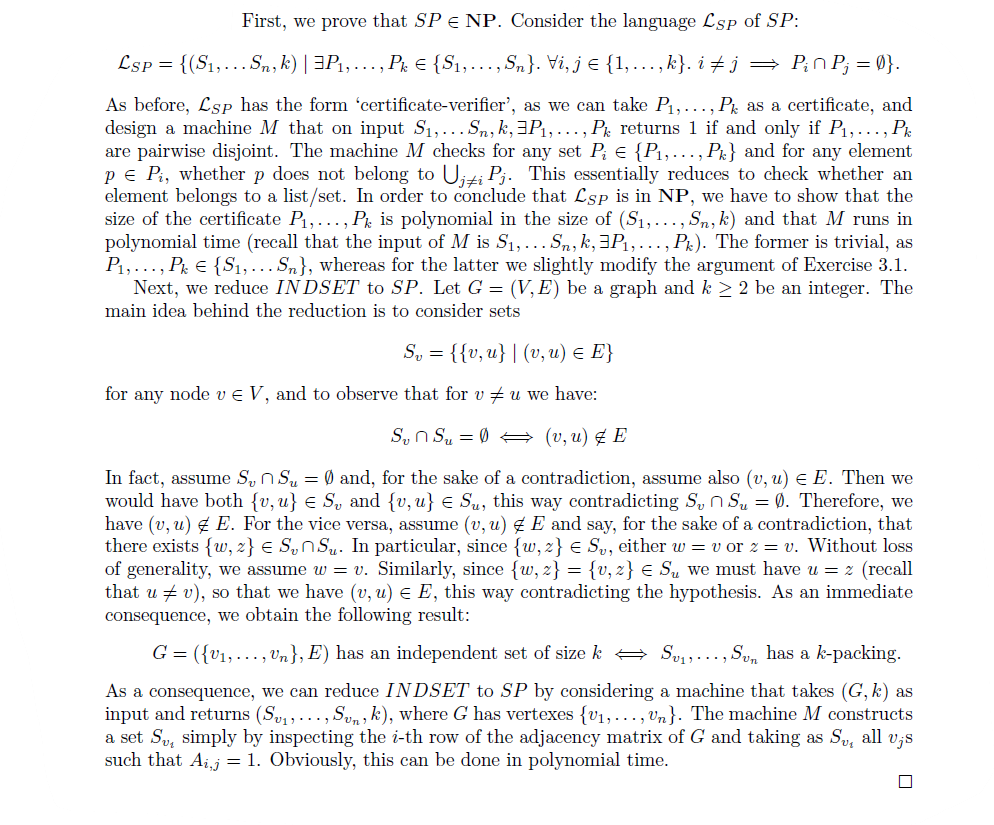
\includegraphics[scale=0.8]{figures/old/SP}}
	% \end{figure}
\end{ex}



% \section{Theory exercises (with solutions)}
%  \begin{figure}[H]
% \centerline{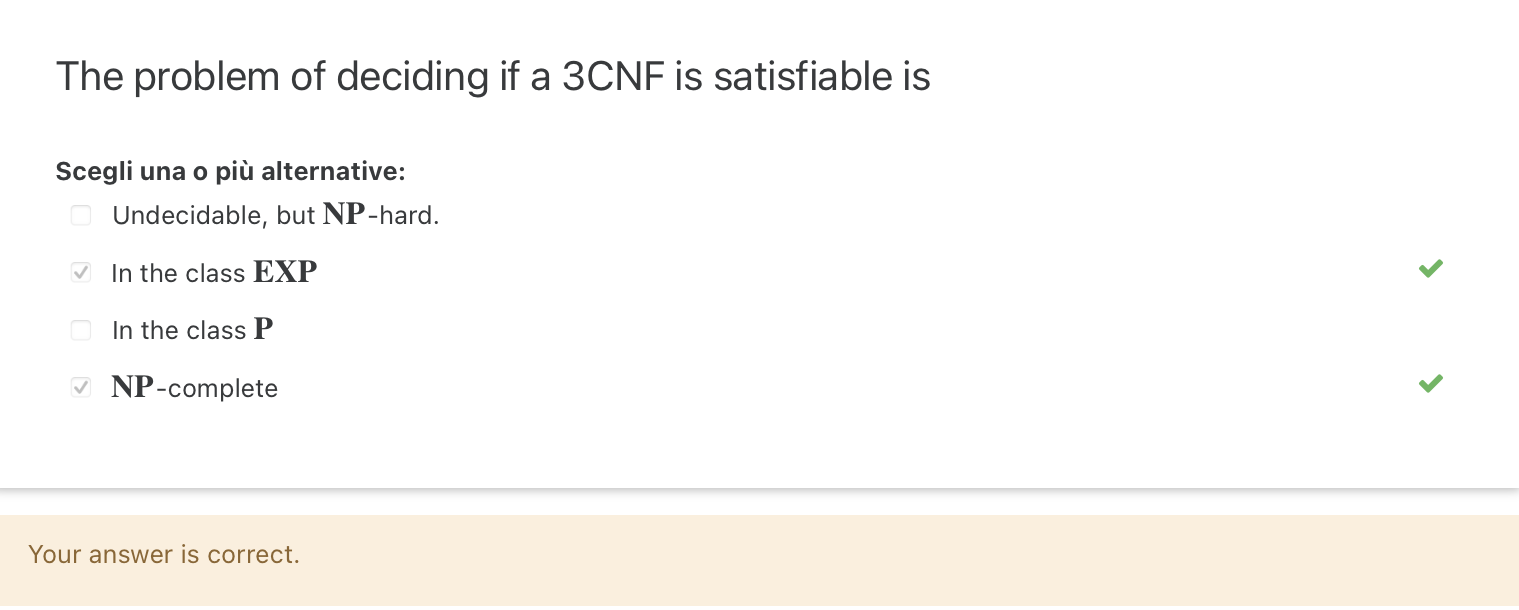
\includegraphics[scale=0.5]{figures/old/theory/1}}
% \end{figure}
%  \begin{figure}[H]
% \centerline{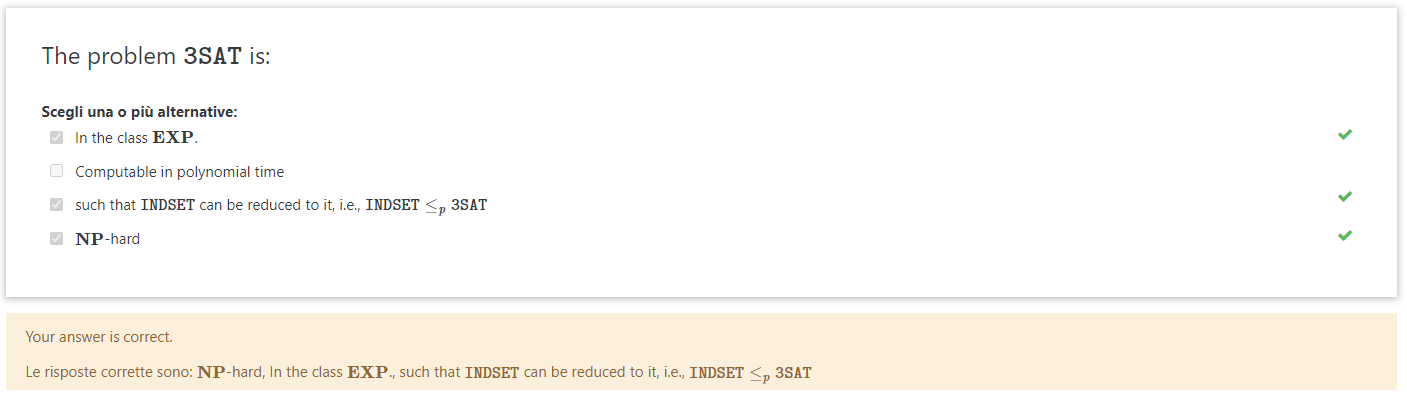
\includegraphics[scale=0.5]{figures/old/theory/2}}
% \end{figure}
%  \begin{figure}[H]
% \centerline{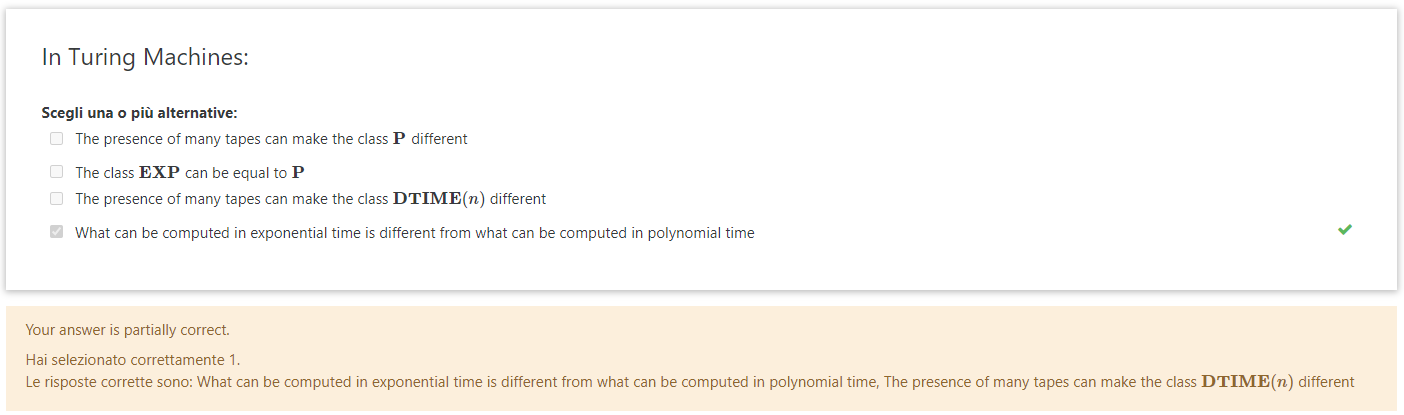
\includegraphics[scale=0.5]{figures/old/theory/3}}
% \end{figure}
%  \begin{figure}[H]
% \centerline{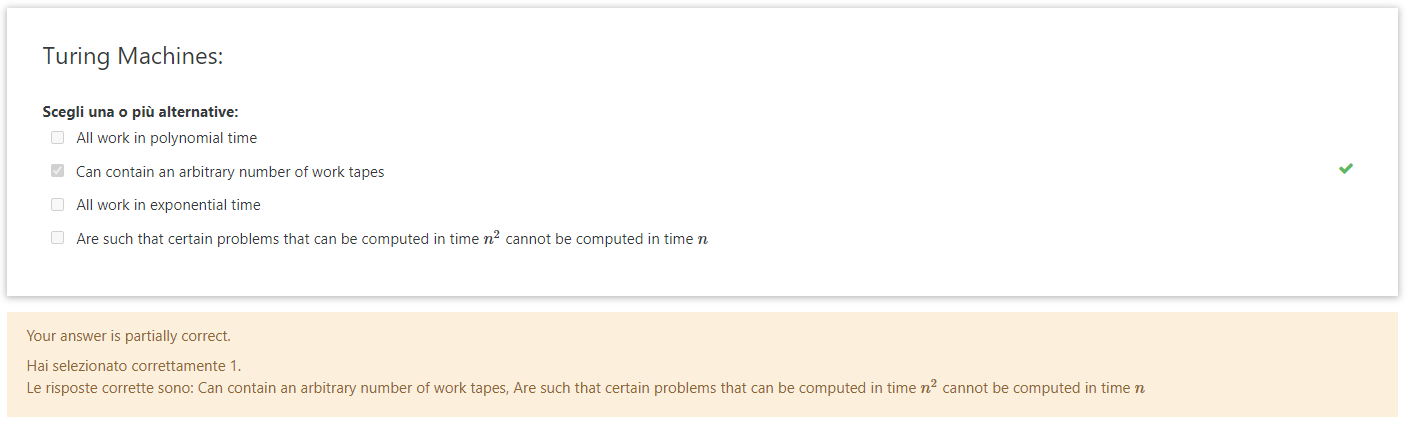
\includegraphics[scale=0.5]{figures/old/theory/4}}
% \end{figure}
%  \begin{figure}[H]
% \centerline{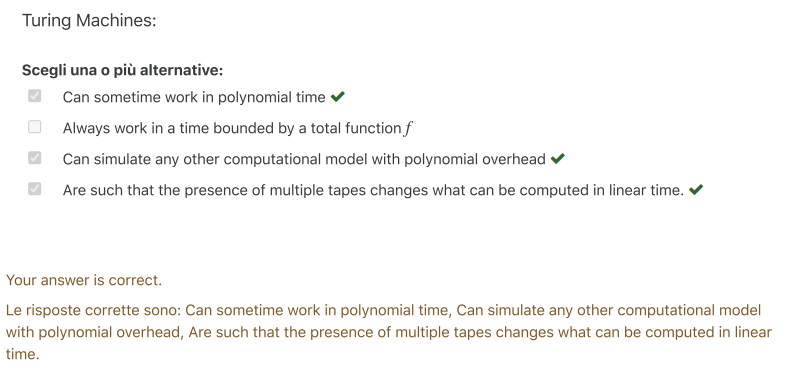
\includegraphics[scale=0.5]{figures/old/theory/5}}
% \end{figure}
%  \begin{figure}[H]
% \centerline{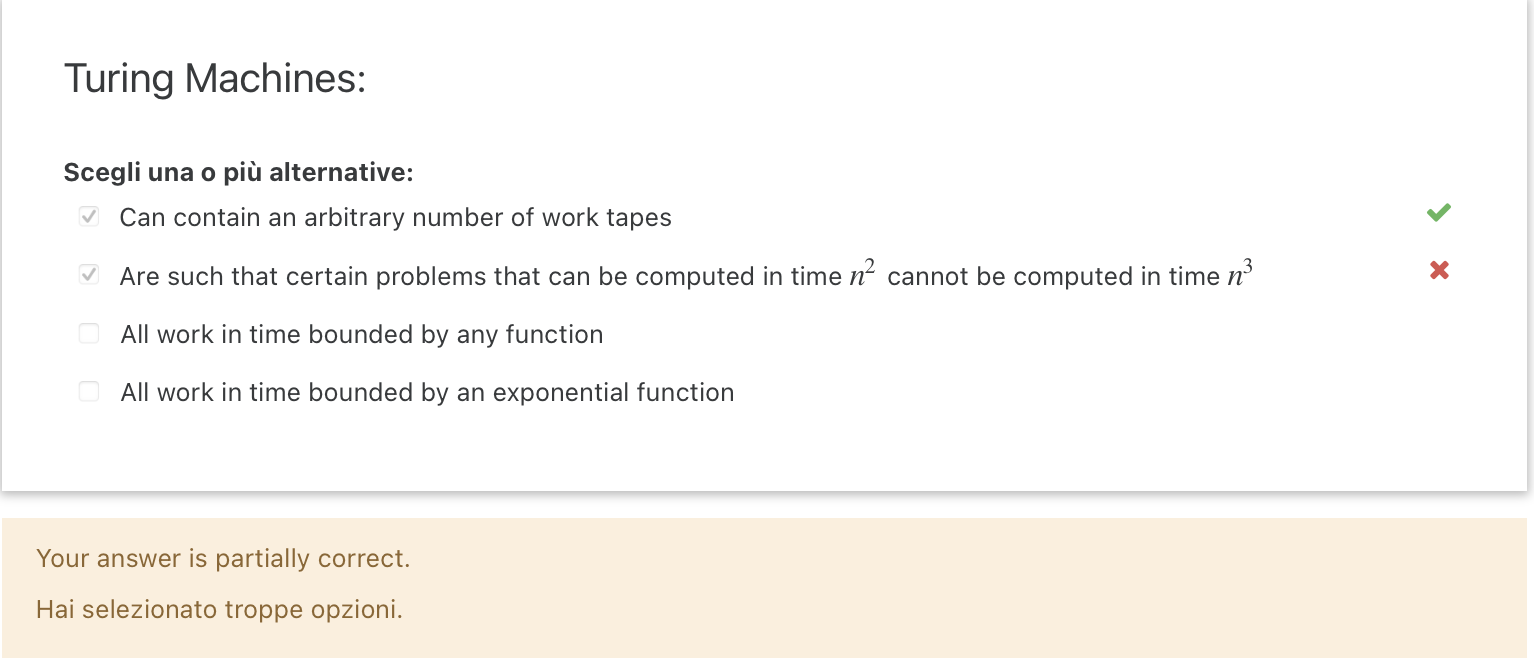
\includegraphics[scale=0.5]{figures/old/theory/6}}
% \end{figure}
%  \begin{figure}[H]
% \centerline{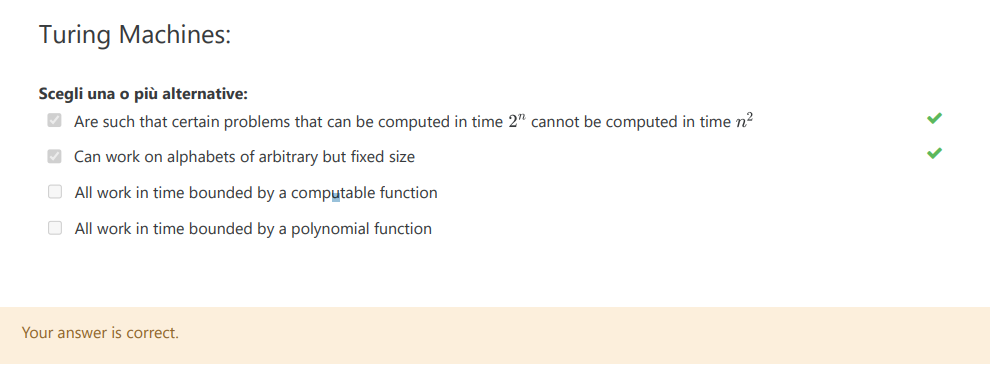
\includegraphics[scale=0.5]{figures/old/theory/7}}
% \end{figure}
%  \begin{figure}[H]
% \centerline{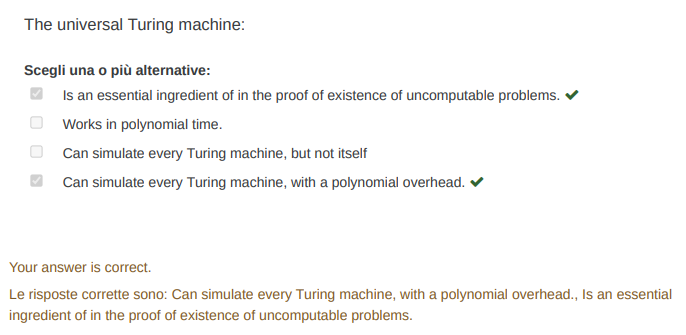
\includegraphics[scale=0.5]{figures/old/theory/8}}
% \end{figure}
%  \begin{figure}[H]
% \centerline{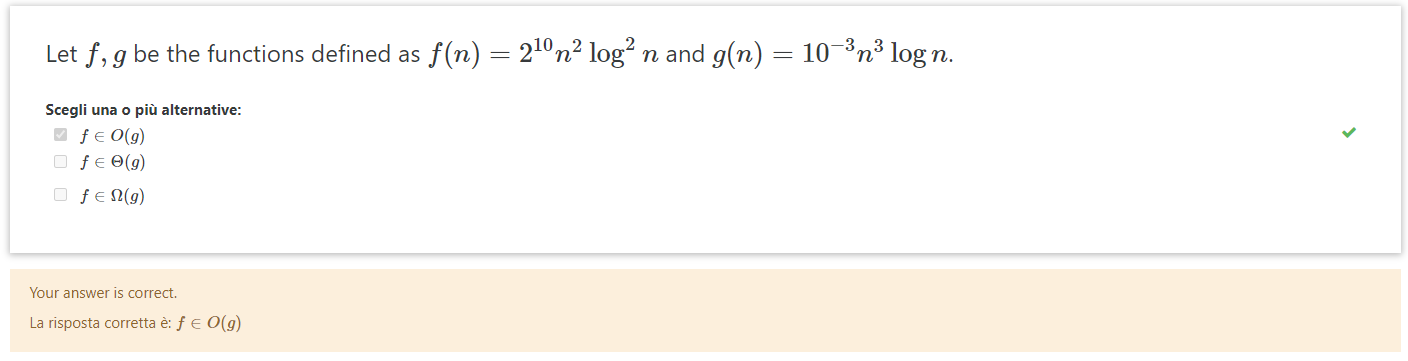
\includegraphics[scale=0.5]{figures/old/theory/9}}
% \end{figure}
%  \begin{figure}[H]
% \centerline{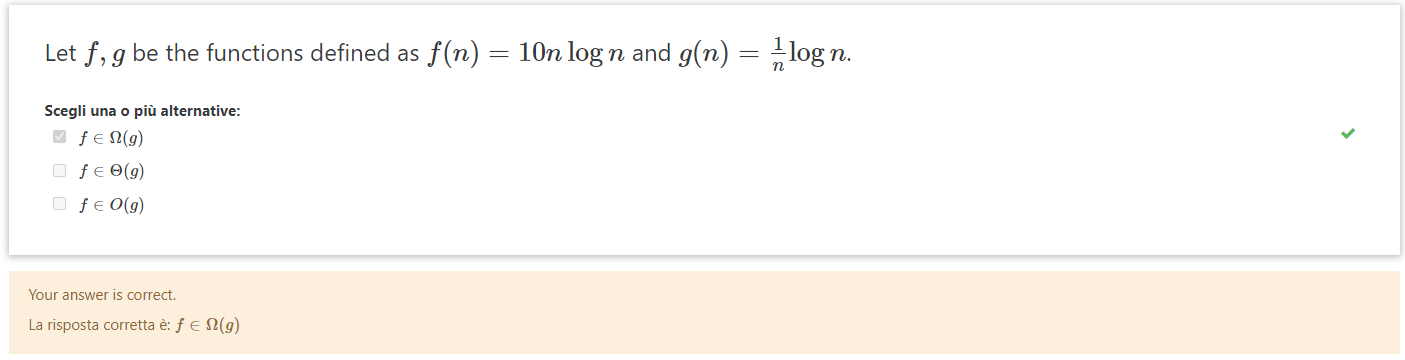
\includegraphics[scale=0.5]{figures/old/theory/10}}
% \end{figure}
%  \begin{figure}[H]
% \centerline{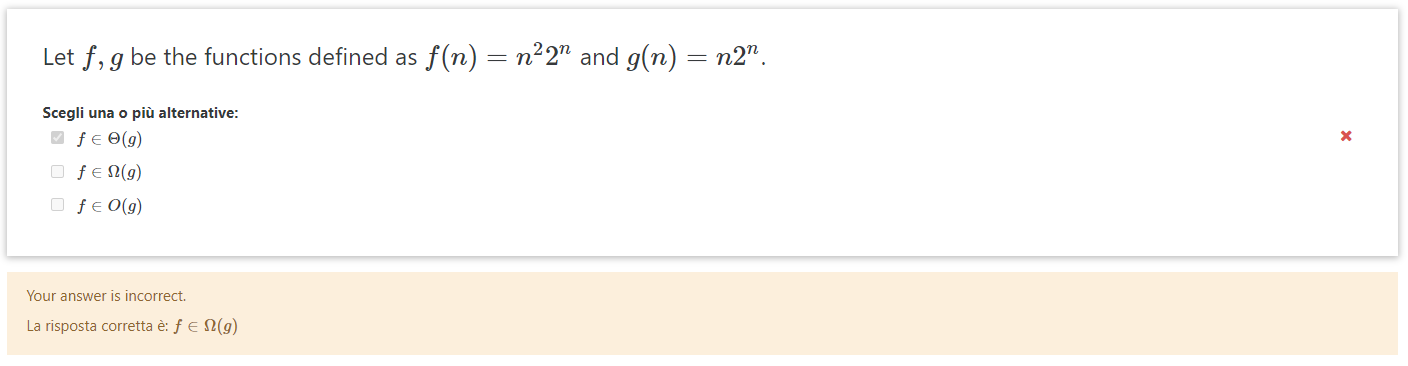
\includegraphics[scale=0.5]{figures/old/theory/11}}
% \end{figure}
%  \begin{figure}[H]
% \centerline{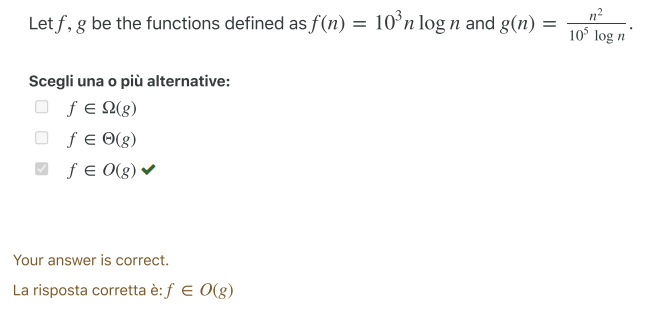
\includegraphics[scale=0.5]{figures/old/theory/12}}
% \end{figure}
%  \begin{figure}[H]
% \centerline{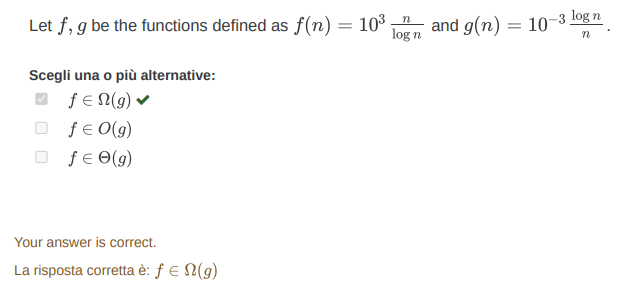
\includegraphics[scale=0.5]{figures/old/theory/13}}
% \end{figure}
%  \begin{figure}[H]
% \centerline{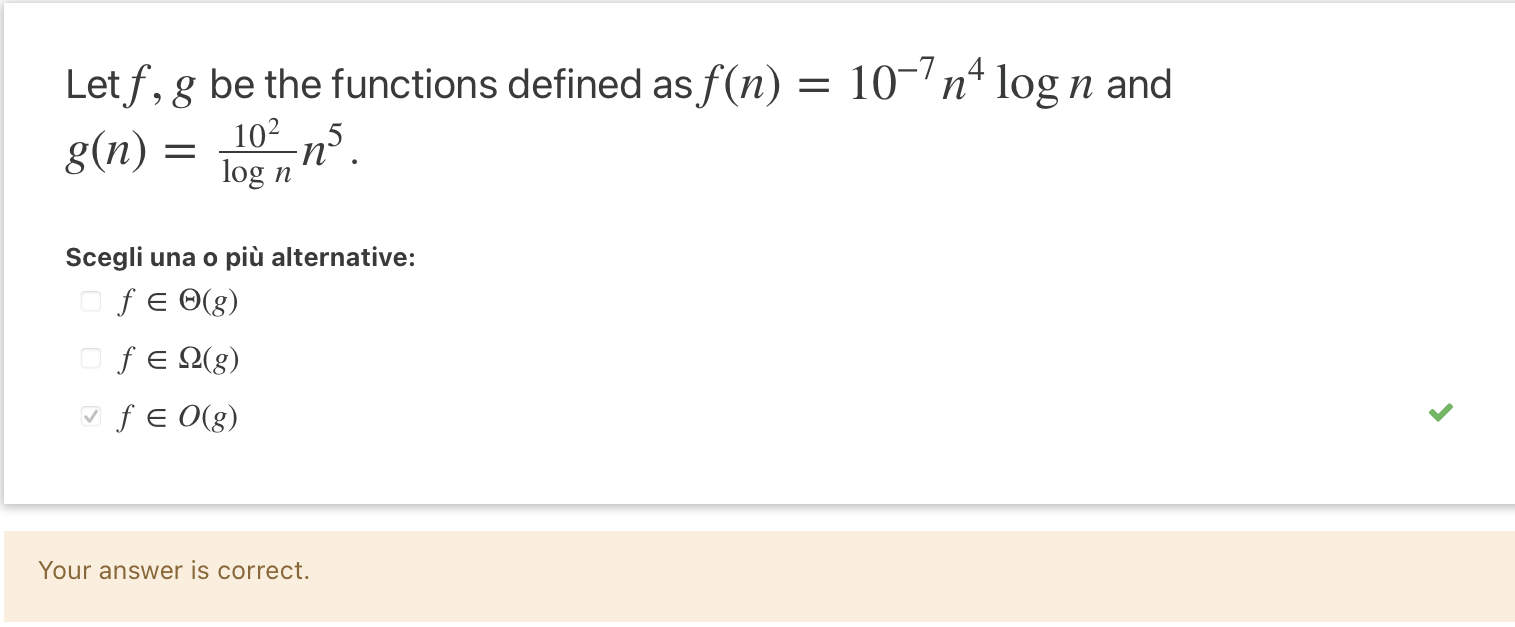
\includegraphics[scale=0.5]{figures/old/theory/14}}
% \end{figure}
%  \begin{figure}[H]
% \centerline{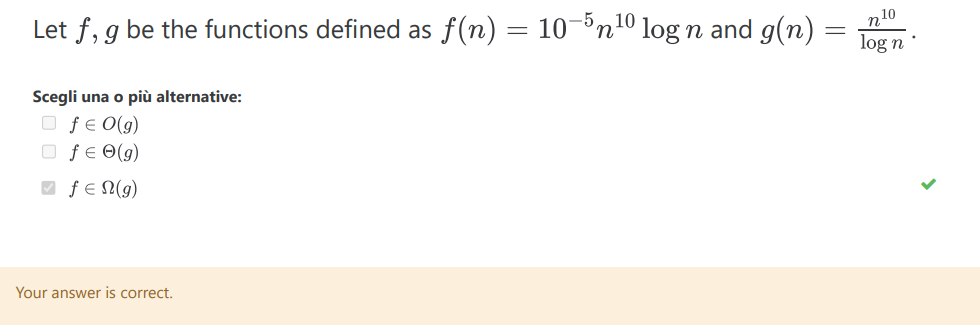
\includegraphics[scale=0.5]{figures/old/theory/15}}
% \end{figure}
%  \begin{figure}[H]
% \centerline{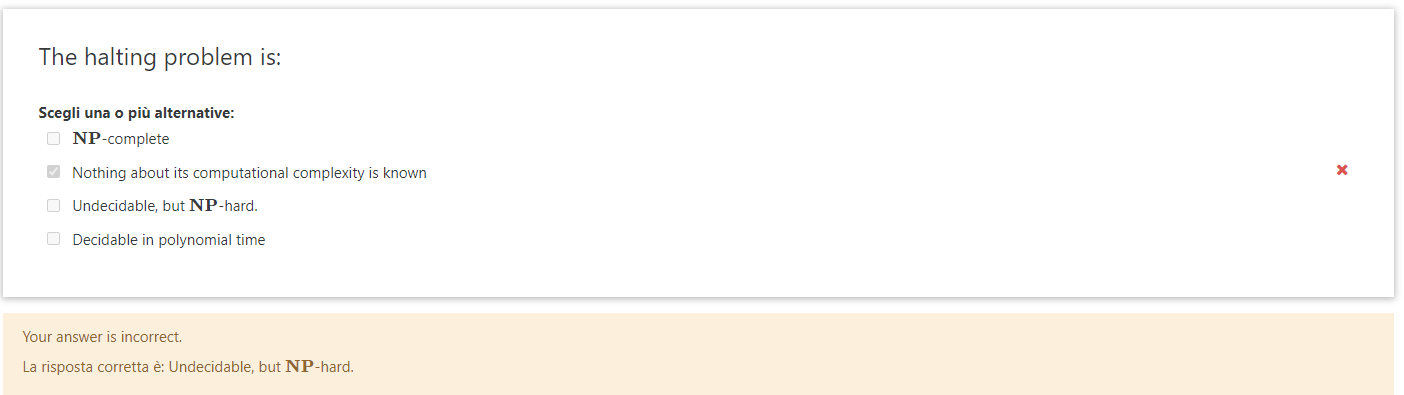
\includegraphics[scale=0.5]{figures/old/theory/16}}
% \end{figure}
%  \begin{figure}[H]
% \centerline{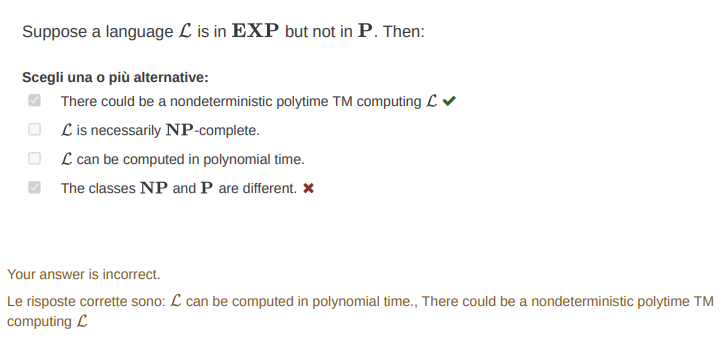
\includegraphics[scale=0.5]{figures/old/theory/17}}
% \end{figure}
%  \begin{figure}[H]
% \centerline{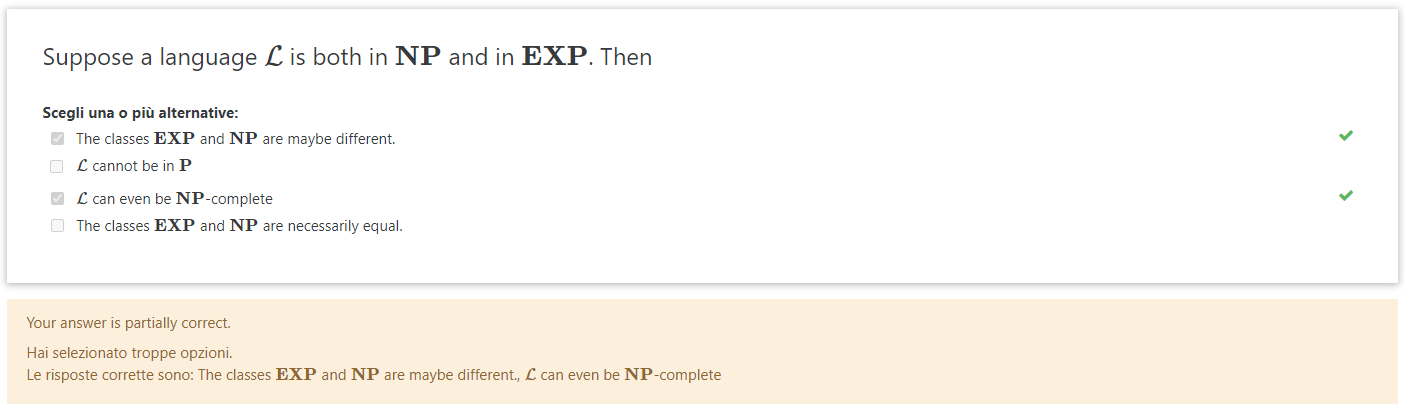
\includegraphics[scale=0.5]{figures/old/theory/18}}
% \end{figure}
%  \begin{figure}[H]
% \centerline{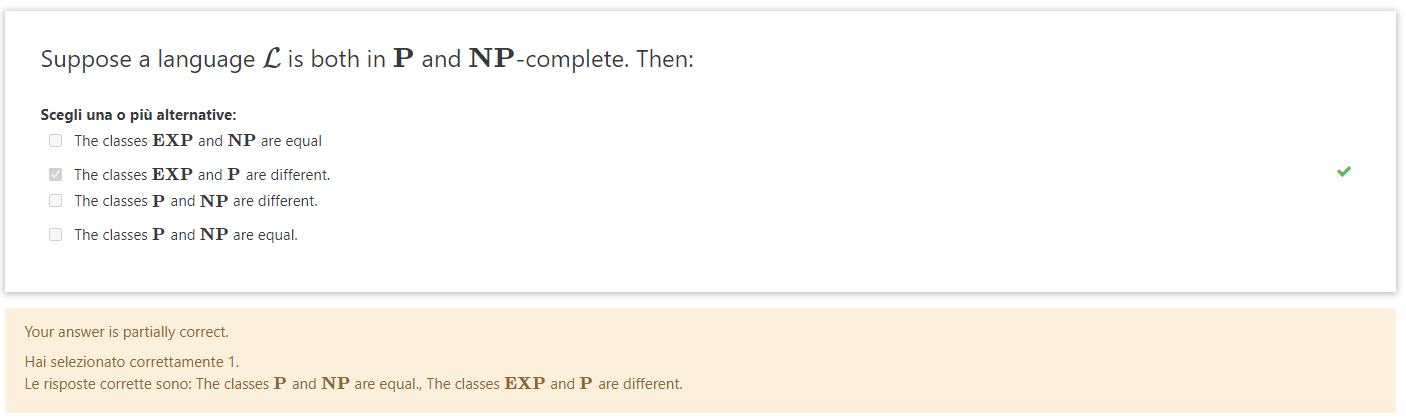
\includegraphics[scale=0.5]{figures/old/theory/19}}
% \end{figure}
%  \begin{figure}[H]
% \centerline{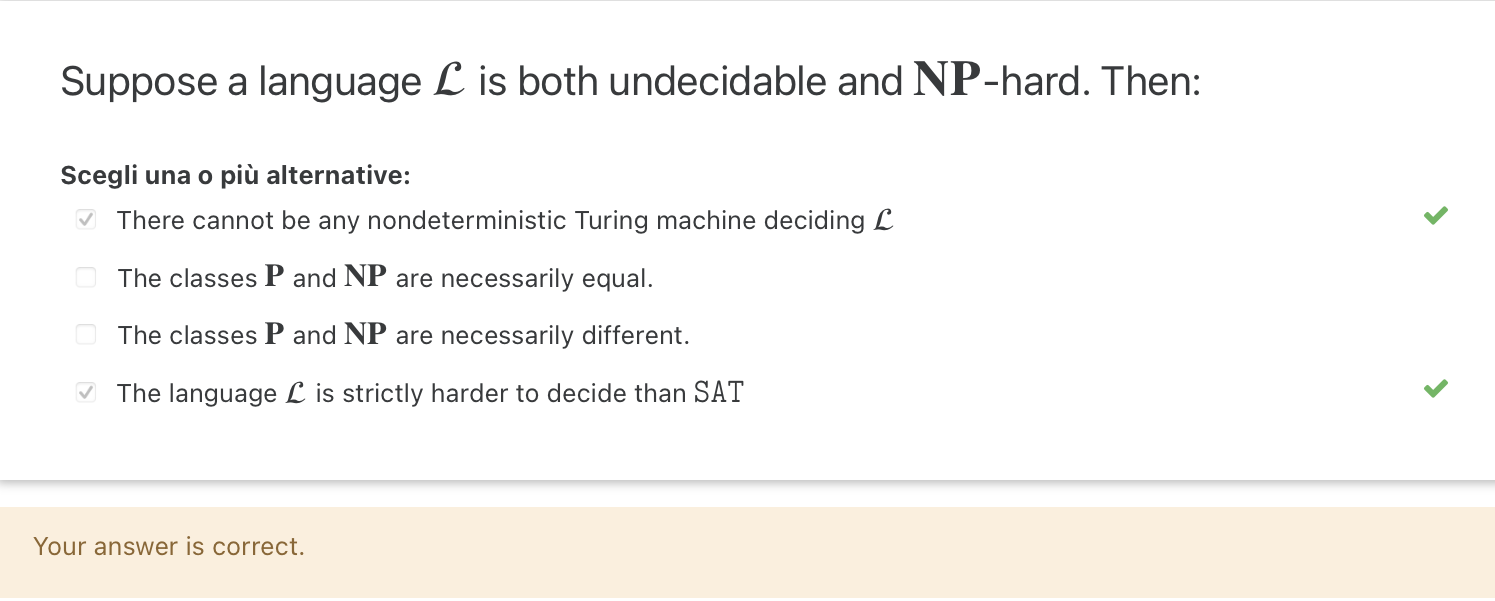
\includegraphics[scale=0.5]{figures/old/theory/20}}
% \end{figure}
%  \begin{figure}[H]
% \centerline{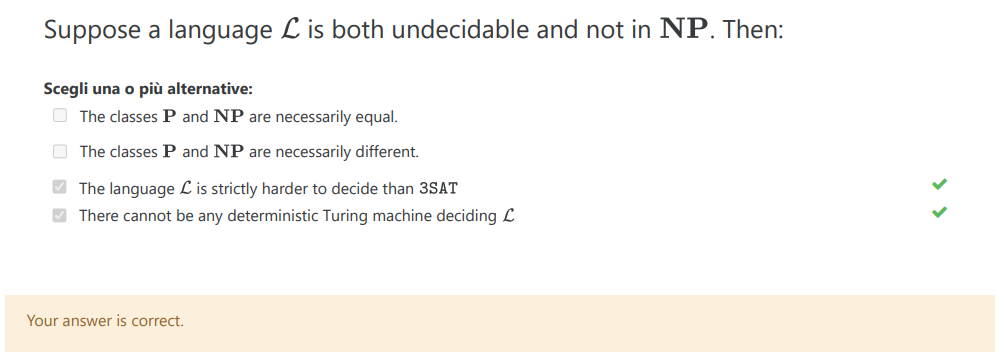
\includegraphics[scale=0.5]{figures/old/theory/21}}
% \end{figure}
%  \begin{figure}[H]
% \centerline{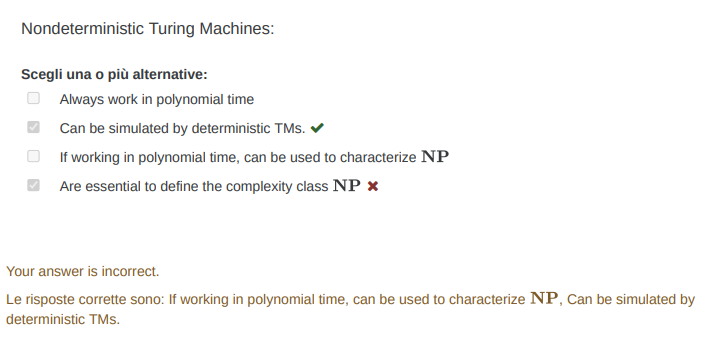
\includegraphics[scale=0.5]{figures/old/theory/22}}
% \end{figure}
%  \begin{figure}[H]
% \centerline{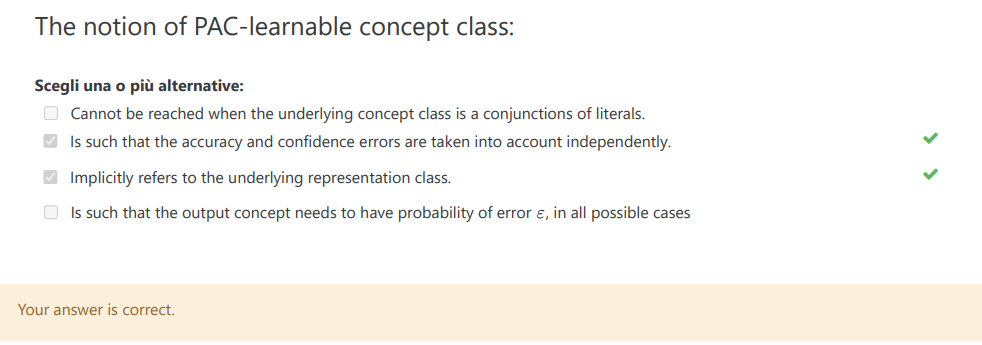
\includegraphics[scale=0.5]{figures/old/theory/23}}
% \end{figure}
%  \begin{figure}[H]
% \centerline{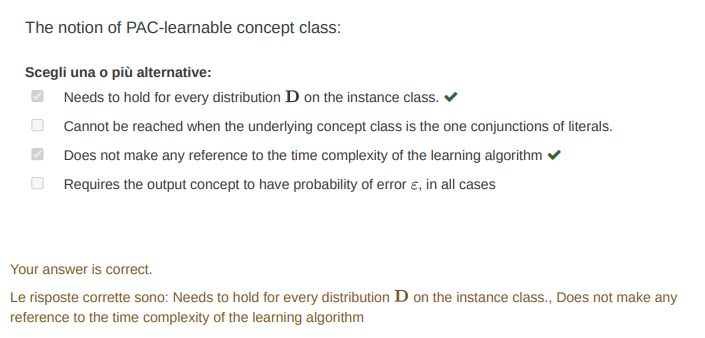
\includegraphics[scale=0.5]{figures/old/theory/24}}
% \end{figure}
%  \begin{figure}[H]
% \centerline{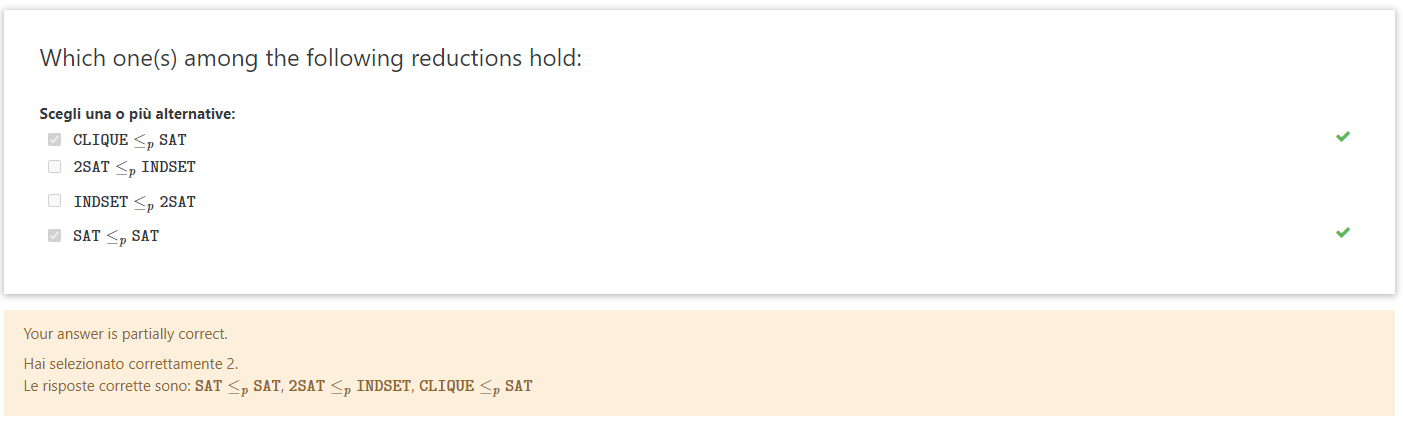
\includegraphics[scale=0.5]{figures/old/theory/25}}
% \end{figure}




